\documentclass{beamer}

\usepackage[english,russian]{babel}
\usepackage[utf8]{inputenc}
%Information to be included in the title page:
\title{Исследование критериев остановки нелинейных решателей при моделировании ненасыщенной фильтрации}
\author{студент 3 курса кафедры вычислительной математики Петрунников Тимур}
\institute{Научный руководитель: к.ф.-м.н. Ануприенко Денис Валерьевич}
\date{2025}

\begin{document}
	
	\frame{\titlepage}
	
	\begin{frame}
		\frametitle{Актуальность задачи}
		\begin{figure}[h] \centering
			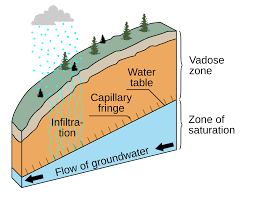
\includegraphics[width=0.4\textwidth]{cap_fringe}
		\end{figure}
		Моделирование ненасыщенной фильтрации:
		\begin{itemize}
			\item При рассмотрении любых приповерхностных объектов, влияющих на подземные воды
			\item Сильная нелинейность уравнения Ричардса: трудности численного решения даже в 1D
			\item Выбор критериев остановки решателей не всегда понятен пользователю
		\end{itemize}
	\end{frame}
	
	
	\begin{frame}
		\frametitle{Цель работы}
		Цель работы -- выявить закономерности в достаточных критериях остановки нелинейных решателей\\
		Для этого необходимо:
		\begin{itemize}
			\item Изучить постановку задачи
			\item Выбрать схему дискретизации и метод решения систем
			\item Программно реализовать эти подходы
			\item Провести численные эксперименты
		\end{itemize}
	\end{frame}
	
	
	
	\begin{frame}
		\frametitle{Постановка задачи}
		Уравнение Ричардса + ГУ + НУ:
		\begin{equation*}\label{eq:ivp_richards_1d}
			\begin{cases}
					\frac{\partial \theta(h)}{\partial t} + S(h)
				s_{stor}(x)\frac{\partial h}{\partial t} + \frac{\partial q}{\partial x} = 0, ~ x \in (0,L), ~ t\in(0, t_{\max})\\
				q = -K_r(h)K(x)\frac{\partial h}{\partial x},\\
				h(0,t) = H_0,~~h(L,t) = H_L,\\
				h(x,0) = H_{init}(x)
			\end{cases}
		\end{equation*}
		где
		\begin{itemize}
			\item $h$ -- напор воды, основная неизвестная
			\item $q$ -- поток
			\item $\theta(h)$ -- влагосодержание, нелинейная функция
			\item $S(h) = \theta(h)/\theta_s$ -- насыщенность
			\item $K(x)$ -- коэффициент фильтрации
			\item $K_r(h)$ -- относительная проницаемость, нелинейная функция
			\item $s_{stor}(x)$ -- коэффициент упругой емкости.
		\end{itemize}
	\end{frame}
	
	
	\begin{frame}
		\frametitle{Дискретизация}
		По пространству
		\begin{itemize}
			\item Метод конечных объемов на равномерной сетке
			\item Напоры в ячейках, потоки в узлах
			\item Локальная консервативность
		\end{itemize}
		
		
		По пространству
		\begin{itemize}
			\item Неявная схема
			\item Абсолютная устойчивость
			\item Необходимость решать систему алгебраических уравнений
		\end{itemize}
	\end{frame}
	
	
	\begin{frame}
		\frametitle{Метод конечных объемов}
		По пространству
		\begin{itemize}
			\item Метод конечных объемов на равномерной сетке
			\item Напоры в ячейках, потоки в узлах
			\item Локальная консервативность
		\end{itemize}
		
		
		По пространству
		\begin{itemize}
			\item Неявная схема
			\item Абсолютная устойчивость
			\item Необходимость решать систему алгебраических уравнений
		\end{itemize}
	\end{frame}
	
	\begin{frame}
	\frametitle{Метод конечных объемов}
	\begin{figure}[h] \centering
		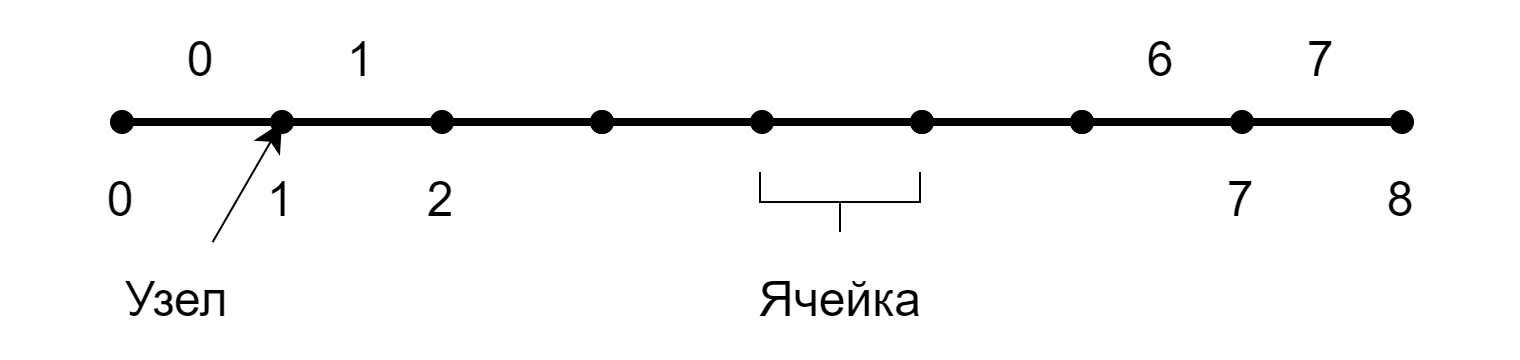
\includegraphics[width=0.8\textwidth]{mesh1d}
	\end{figure}
	Интегрируем уравнение по ячейке  $[x_i, x_{i+1}]$:
	
	\begin{equation*}
		\int_{x_i}^{x_{i+1}}\left[ \frac{\partial \theta(h)}{\partial h}
		\frac{\partial h}{\partial t} + S(h)s_{stor}(x)\frac{\partial h}{\partial t}
		+
		\frac{\partial q}{\partial x}
		\right]dx = 0
	\end{equation*}
	Производные по времени аппроксимируются неявной схемой:
	\begin{equation*}
		\int_{x_i}^{x_{i+1}}\left[ \frac{\partial \theta(h)}{\partial h}
		\frac{\partial h}{\partial t} + S(h)s_{stor}(x)\frac{\partial h}{\partial t}
		\right]dx \approx
	\end{equation*}
	\begin{equation*}\left[ \frac{\partial \theta(h^{n+1}_i)}{\partial h}
		\frac{h_i^{n+1} - h_i^{n}}{\Delta t} + S(h_i^{n+1})s_{stor}(x)\frac{h_i^{n+1} - h_i^n}{\Delta t}
		\right]\Delta x
	\end{equation*}
	\end{frame}
	
	
	
	\begin{frame}
		\frametitle{Метод конечных объемов}
		\begin{figure}[h] \centering
			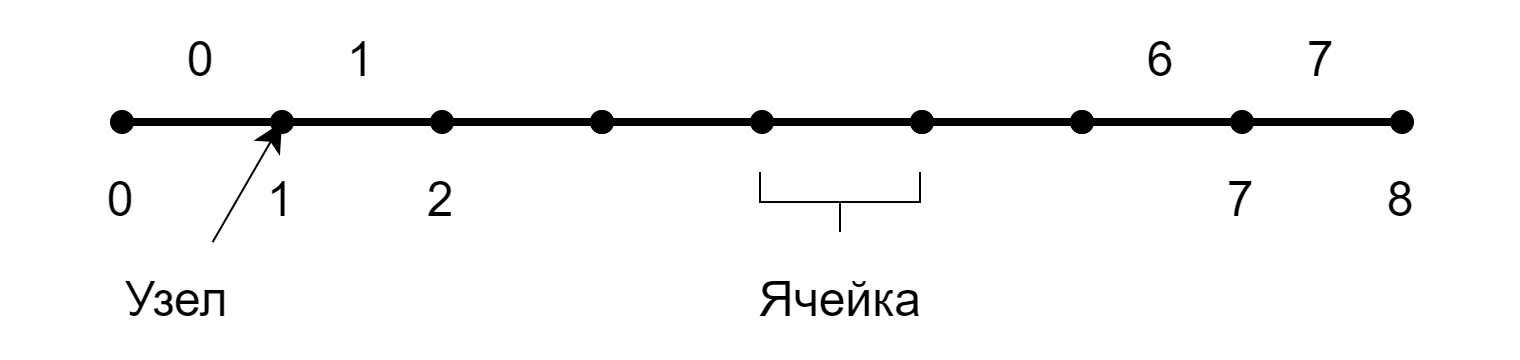
\includegraphics[width=0.8\textwidth]{mesh1d}
		\end{figure}
		
		В итоге имеем
		\begin{equation*}\left[ \frac{\partial \theta(h^{n+1}_i)}{\partial h}
			\frac{h_i^{n+1} - h_i^{n}}{\Delta t} + S(h_i^{n+1})s_{stor}(x)\frac{h_i^{n+1} - h_i^n}{\Delta t}
			\right]\Delta x + q_{i+1}^{n+1} - q_i^{n+1} = 0.
		\end{equation*}
		
		Потоки вычисляются конечными разностями
		
		\begin{equation*}
			q_i = \frac{2K_iK_{i-1}}{K_i + K_{i-1}}K_r(h_{upw})\frac{h_i - h_{i-1}}{\Delta x}.
		\end{equation*}
	\end{frame}
	
	\begin{frame}
	\frametitle{Решение нелинейных систем}
	Разностная схема представляет собой систему нелинейных алгебраических уравнений вида
	\begin{equation*}
		A(h^{n+1})h^{n+1} = b(h^{n+1}),
	\end{equation*}
	где матрица $A$ -- трехдиагональная.
	
	Для решения используется метод простой итерации:
	
	\begin{equation*}
		A(h^{n+1,k})h^{n+1,k+1} = b(h^{n+1,k}),
	\end{equation*}
	итерации останавливаются при
	
	\begin{equation*}
		||r_k|| < \varepsilon_{rel}||r_0||\text{~или~} ||r_k||<\varepsilon_{abs}
	\end{equation*}
	Как выбирать эти критерии $\varepsilon_{rel}, \varepsilon_{abs}$ на практике? Как они зависят от параметров задачи?
	\end{frame}
	
	
	\begin{frame}
	\frametitle{Численные эксперименты}
	\begin{itemize}
		\item Втекание воды в колонку из сухого грунта
		\item Четкий фронт решения
		\item Как критерий $\varepsilon_{abs}$ влияет на положение фронта?
	\end{itemize}
	Для наглядной демонстрации приводятся решения при $\varepsilon_{abs} = 10^{-7}$, $\varepsilon_{abs} = 0.1$ для разных сеток
	\end{frame}
	
	\begin{frame}
		\frametitle{Численные эксперименты}
		\begin{figure}[h] \centering
			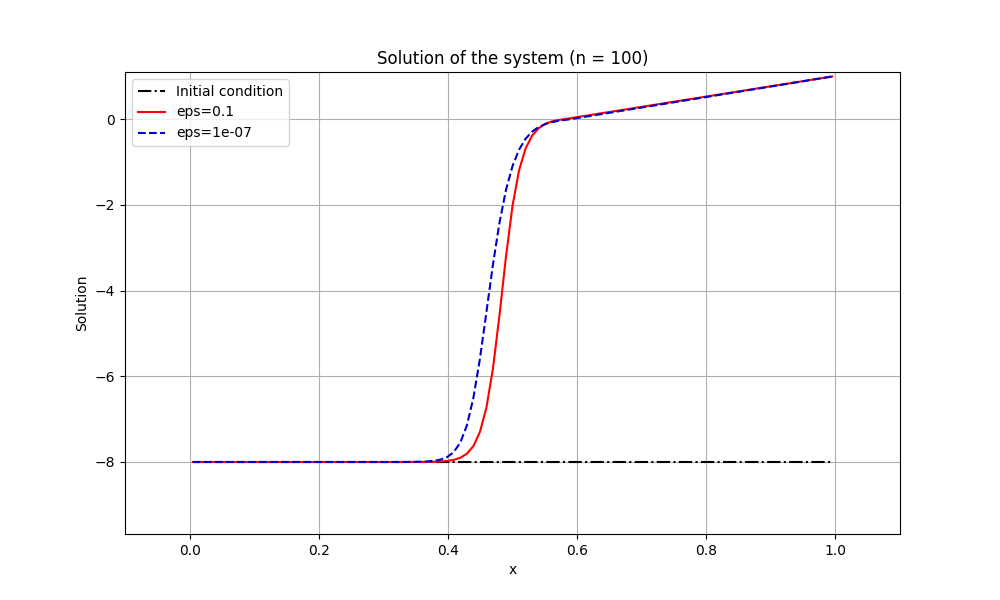
\includegraphics[width=1\textwidth]{n100}
		\end{figure}
		С измельчением сетки $\varepsilon_{abs} = 0.1$ приводит к все худшим решениям
	\end{frame}
	
	\begin{frame}
	\frametitle{Численные эксперименты}
	\begin{figure}[h] \centering
		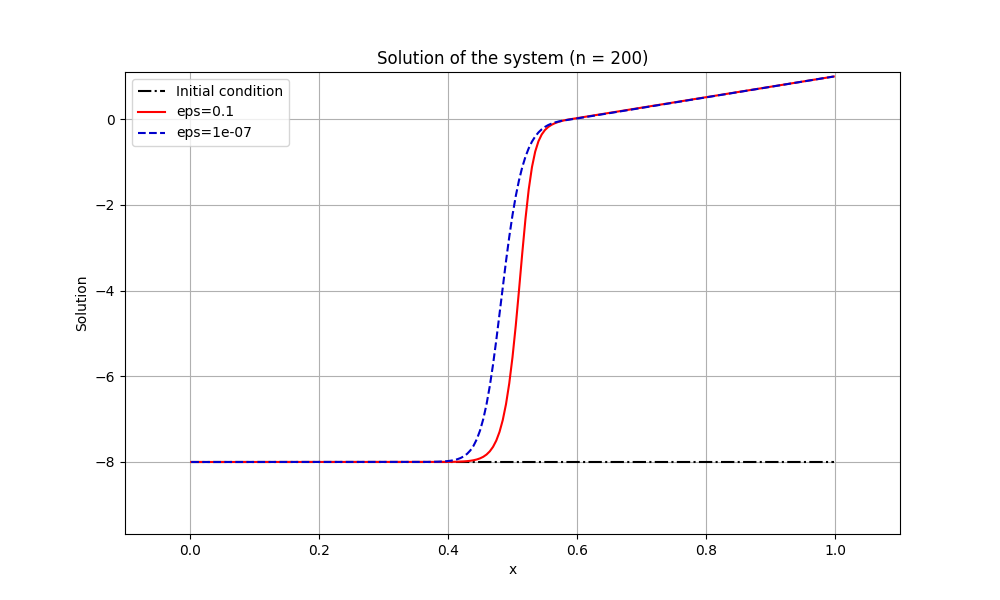
\includegraphics[width=1\textwidth]{n200}
	\end{figure}
	С измельчением сетки $\varepsilon_{abs} = 0.1$ приводит к все худшим решениям
	\end{frame}
	
	\begin{frame}
	\frametitle{Численные эксперименты}
	\begin{figure}[h] \centering
		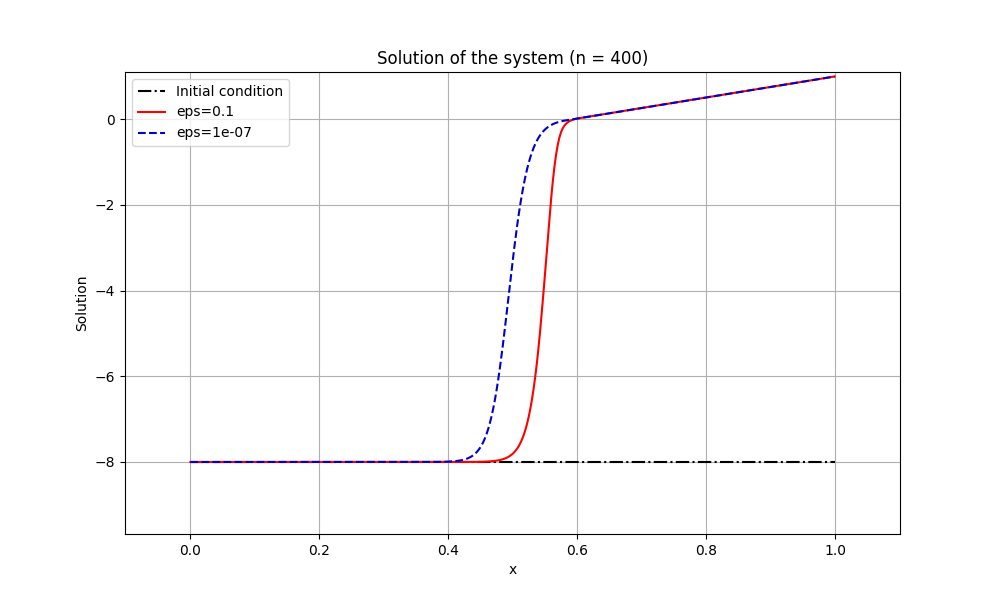
\includegraphics[width=1\textwidth]{n400}
	\end{figure}
	С измельчением сетки $\varepsilon_{abs} = 0.1$ приводит к все худшим решениям
	\end{frame}
	
	\begin{frame}
	\frametitle{Численные эксперименты}
	\begin{figure}[h] \centering
		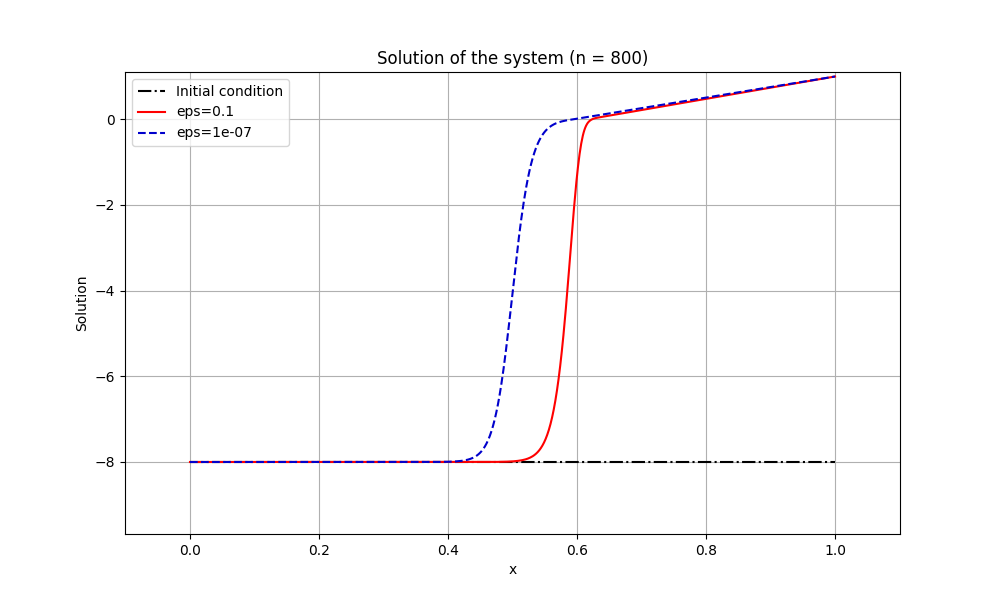
\includegraphics[width=1\textwidth]{n800}
	\end{figure}
	С измельчением сетки $\varepsilon_{abs} = 0.1$ приводит к все худшим решениям
	\end{frame}
	
	\begin{frame}
	\frametitle{Заключение}
	\begin{itemize}
		\item Изучена постановка задачи ненасыщенной фильтрации на основе уравнения Ричардса
		\item Построена неявная схема дискретизации методом конечных объемов
		\item Программно реализовано решение на ЯП Python
		\item Экспериментально установлена зависимость достаточно критерия остановки от шага сетки
	\end{itemize}
	\end{frame}
	
		\begin{frame}
		\frametitle{}
		\centering\Large Спасибо за внимание!
	\end{frame}
	
\end{document}